%%%%%%%%%%%%%%%%%%%%%%%%%%%%%%%%%%%%%%%%%
% a0poster Landscape Poster
% LaTeX Template
% Version 1.0 (22/06/13)
%
% The a0poster class was created by:
% Gerlinde Kettl and Matthias Weiser (tex@kettl.de)
% 
% This template has been downloaded from:
% http://www.LaTeXTemplates.com
%
% License:
% CC BY-NC-SA 3.0 (http://creativecommons.org/licenses/by-nc-sa/3.0/)
%
%%%%%%%%%%%%%%%%%%%%%%%%%%%%%%%%%%%%%%%%%

%----------------------------------------------------------------------------------------
%	PACKAGES AND OTHER DOCUMENT CONFIGURATIONS
%----------------------------------------------------------------------------------------

\documentclass[a0, landscape]{a0poster}


\usepackage{multicol} % This is so we can have multiple columns of text side-by-side
\columnsep=25pt % This is the amount of white space between the columns in the poster
%\columnseprule=3pt % This is the thickness of the black line between the columns in the poster
%\usepackage{graphicx}
%\usepackage{pstricks,pst-grad}
\usepackage[svgnames]{xcolor} % Specify colors by their 'svgnames', for a full list of all colors available see here: http://www.latextemplates.com/svgnames-colors
\usepackage{setspace}
%\definecolor{DarkSlateBlue}{RGB}{179, 27, 27} % UBC Blue (primary)


\usepackage{titlesec}
\titlespacing*{\section}
{0pt}{3.0ex minus .2ex}{2.3ex plus .2ex}
\titlespacing*{\subsection}
{0pt}{3.0ex minus .2ex}{2.3ex plus .2ex}
%\renewcommand{\familydefault}{\sfdefault}
%\usepackage[scaled=1]{helvet}
%\usepackage[helvet]{sfmath}
%\everymath={\sf}
%\usepackage{times} % Use the times font
%\usepackage{helvet}
%\usepackage{palatino} % Uncomment to use the Palatino font
%\usepackage[times]{sfmath}
\usepackage{graphicx} % Required for including images
\usepackage{pstricks,pst-grad}
\graphicspath{{figures/}} % Location of the graphics files
\usepackage{booktabs} % Top and bottom rules for table
\usepackage[font=small,labelfont=bf]{caption} % Required for specifying captions to tables and figures
\usepackage{amsfonts, amsmath, amsthm, amssymb} % For math fonts, symbols and environments
\usepackage{wrapfig} % Allows wrapping text around tables and figures
\usepackage{natbib}

\usepackage{tikz}

% Definition of \boxed in amsmath.sty:
% \newcommand{\boxed}[1]{\fbox{\m@th$\displaystyle#1$}}

% Syntax: \colorboxed[<color model>]{<color specification>}{<math formula>}
\newcommand*{\colorboxed}{}
\def\colorboxed#1#{%
  \colorboxedAux{#1}%
}
\newcommand*{\colorboxedAux}[3]{%
  % #1: optional argument for color model
  % #2: color specification
  % #3: formula
  \begingroup
    \colorlet{cb@saved}{.}%
    \color#1{#2}%
    \boxed{%
      \color{cb@saved}%
      #3%
    }%
  \endgroup
}

\usepackage{xcolor}

\begin{document}

\begin{tikzpicture}[remember picture, overlay]
     \node [anchor=north east, inner sep=3cm]  at (current page.north east)
     {
\includegraphics[height=7.5cm]{logo}};
 \end{tikzpicture}

%----------------------------------------------------------------------------------------
%	POSTER HEADER 
%----------------------------------------------------------------------------------------

% The header is divided into three boxes:
% The first is 55% wide and houses the title, subtitle, names and university/organization
% The second is 25% wide and houses contact information
% The third is 19% wide and houses a logo for your university/organization or a photo of you
% The widths of these boxes can be easily edited to accommodate your content as you see fit
%\begin{minipage}[b]{0.09\linewidth}
%
\includegraphics[width=10cm]{logo.png} % Logo or a photo of you, %adjust its dimensions here
%\end{minipage}

\begin{minipage}{\linewidth}
\begin{center}
\linespread{1.5}
\color{DarkSlateBlue} \Huge \textbf{Normality of Toric Rings and Rees Algebras of Pinched Strongly Stable Ideals}

 \color{Black}
\LARGE  Cameron Chandler, Margit Liu, Elizabete Mezinska, Andrew Moore, Shashank Sule, Andrew Tawfeek

 % Author(s)

\LARGE  Advisor: Gabriel Sosa % University/organization    
\end{center}
\end{minipage}
    


%
%\begin{minipage}[b]{0.25\linewidth}
%\color{DarkSlateGray}\Large \textbf{Contact Information:}\\
%Department Name\\ % Address
%University Name\\
%123 Broadway, State, Country\\\\
%Phone: +1 (000) 111 1111\\ % Phone number
%Email: \texttt{john@LaTeXTemplates.com}\\ % Email address
%\end{minipage}
%
%\begin{minipage}[b]{0.09\linewidth}
 % Logo or a photo of you, %adjust its dimensions here
%\end{minipage}

\vspace{1cm} % A bit of extra whitespace between the header and poster content
  \hline
\vspace{1cm}
%----------------------------------------------------------------------------------------

\begin{multicols}{4} % This is how many columns your poster will be broken into, a poster with many figures may benefit from less columns whereas a text-heavy poster benefits from more




%----------------------------------------------------------------------------------------
%	INTRODUCTION
%----------------------------------------------------------------------------------------

%\color{SaddleBrown} % SaddleBrown color for the introduction

\section*{\color{DarkSlateBlue}Introduction}

%Let $K$ be an algebraically closed field. Then a \textbf{Toric ring} is defined as a subring $K[T] \subset K[x_1, \ldots, x_n] $  where $T$ is a set of monomials, i.e $T = \{ \mathbf{x_1}^\mathbf{\alpha_1}, \ldots, \mathbf{x_s}^\mathbf{\alpha_s}\}$. For example, $K[x^2,  xy,  xz,  y^2]$, which  is a subring  of $K[x, y, z]$, is a toric ring. 

%Toric rings are central objects within commutative algebra and have been studied for their properties since the days of the renaissance. In our project, we were interested in the \textit{Normality} of special types of toric rings. A toric ring is \textit{normal} when all rational solutions of monic equations are elements of the ring. 

%For example, $\mathbb{Z}$ is normal because all rational solutions of polynomial equations of the form 
%\[x^n+a_{n-1}x^{n-1}+\dots+ a_{1}x+a_{0}=0\]
%where $a_0,a_1,a_2, \dots, a_{n-1} \in \ZZ$ are also integral solutions. 

It is known from the 16th century that the toric ring
$K[x^3, x^2y, xy^2, y^3, x^2z, y^2z, xz^2, yz^2, z^3]$ also called the pinched Veronese, is not normal. Sturmfels \citep{Sturmfels1996} proved that Veronese-type toric rings are normal. Further results from Conca and De Negri \citep{Negri1999} \citep{Bruns2017} show that toric rings of principal Borel ideals are also normal. Motivated by these inquiries, we set out to investigate toric rings generated by pinchings of principal Borel ideals. 

%----------------------------------------------------------------------------------------
%	Methods and Notation
%----------------------------------------------------------------------------------------

%\color{DarkSlateGray} % DarkSlateGray color for the rest of the content

\section*{\color{DarkSlateBlue}Methods and Notation}

Note that these may also be found in \citep{DiPasquale2017}.

\begin{definition}{Toric Ring}\label{Toric Ring}\\
	A \emph{toric ring} is defined as a subring $K[T] \subset K[x_1, \ldots, x_n] $  where $T$ is a set of monomials, i.e $T = \{ \mathbf{x_1}^{\mathbf{a}_1}, \ldots, \mathbf{x_s}^{\mathbf{a}_s}\}$. An example of a toric ring is $K[x^2,  xy,  xz,  y^2]$, which  is a subring  of $K[x, y, z]$.
\end{definition}

\begin{definition}{Normality}\label{Normality}\\
	Let $R$ be a ring and $\bar{R}$ the set of all rational solutions to monic equations with coefficients in $R$. Then $R$ is \emph{normal} if and only if $R = \bar{R}$. For instance, $\mathbb{Z}$ is normal because all rational solutions to monic equations with coefficients in $\mathbb{Z}$ are contained in $\mathbb{Z}$. This is  one of the fundamental results of algebra: \textit{Gauss' Lemma}.
\end{definition}
\begin{definition}{Borel Moves and Borel Ideals}\label{BorelMovesAndIdeals}\\
     A \textit{Borel move} is an operation that sends $m$ to a monomial $\frac{x_j m}{x_i}$ where $ x_i \ | \ m$ and $j \leq i$. A monomial ideal $B$ is a \textit{Borel ideal} if $B$ is generated by a set that is closed under Borel moves. Such a set is called a \textit{Borel set}.
\end{definition}

\begin{definition}{Principal Borel Ideals and Pinchings}\label{PBorelsAndPinchings}\\
The \textit{principal Borel ideal} generated by a monomial $u$ is the ideal $\langle B(u) \rangle$ where $B(u)$ is the minimal strongly stable set of monomials containing $u$.
For example, let $u = b^2c$. Then $I=\langle B(b^2c)\rangle=\langle a^3,a^2b,ab^2,b^3,a^2c,abc,b^2c\rangle$. We say that $\langle B(b^2c) \setminus a^2c\rangle=\langle a^3,a^2b,ab^2,b^3,abc,b^2c\rangle$ is the \textit{pinching} of $a^2c$ from $\langle B(b^2c)\rangle$.
\end{definition}

%\begin{definition}{Borel Graph}\label{Borel Graph}\\
 %The directed graph $G$ is said to be a \textit{Borel Graph} of $B(u)$ if each vertex in $G$ represents a %monomial in $B(u)$. If $m' \in M$ is obtained from a Borel move on $m \in M$, then there is a directed edge f%rom $m$ to $m'$. For example, the Borel Graph of $B(b^2c)$ is as follows:
 
%\begin{center}\vspace{1cm}
%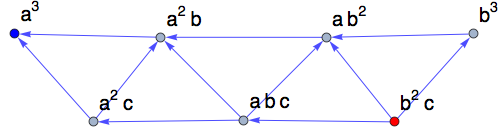
\includegraphics[width=0.8\linewidth]{b2c}
%\captionof{figure}{The Borel Graph of $b^2c$}
%\end{center}\vspace{1cm}
        
%\end{definition}

\begin{definition}{Toric Ideal}\label{Toric Ideal}\\
Let $T = \{m_1, \ldots, m_s\}$ be a set of $s$-many monomials in $K[x_1 \ldots x_n]$ and $K[T]$ be the associated toric ring. Define $\phi$ to be the ring homomorphism 
$$\phi: K[t_1 \ldots t_s] \to K[T]$$
where $\phi(t_i) = m_i$. The \emph{toric ideal} of $K[T]$ is defined to be ker $\phi$.
\end{definition}

\begin{theorem*}\textbf{(Sturmfels)}\cite{Sturmfels1996}\label{Sturmfels} If the minimal generators of in$_<$ker $\phi$ with respect to some monomial ordering $<$ are all squarefree, then $K[T]$ is normal. 
	
\end{theorem*}

The proof can be found in \citep{Ene}. Sturmfels' theorem provides a handy way of discerning the normality of $K[T]$. To put it to effect, we computed (using the computer algebra system, Macaulay2) the initial ideals of the toric ideals of several toric rings of pinched principal Borel ideals and checked them for squarefreeness. 

\begin{goal*}
	Find which pinchings of principal Borel ideals form normal toric rings.
\end{goal*}

%----------------------------------------------------------------------------------------
%	MATERIALS AND METHODS
%----------------------------------------------------------------------------------------

\columnbreak


\section*{\color{DarkSlateBlue}The Main Result}

Before we discuss the main result, we introduce the necessary definitions. Let $\mathcal{H}=\{\mathbf{v}_1,\ldots,\mathbf{v}_s\}$ be a set of vectors in $\mathbb{Z}^n$.

\begin{definition}{Affine Semigroup.}\label{Affine Semigroup}\\
The \textit{affine semigroup} generated by $\mathcal{H}$ is denoted $$\mathbb{N}\mathcal{H} = \left\{ \inline{\sum}_{i=1}^s a_i \mathbf{v}_i \ | \ a_i \in \mathbb{N} \text{ for $1 \leq i \leq s$} \right\}.$$
\end{definition}

\begin{definition}{Affine Group.}\label{Affine group}\\
The \textit{affine group} generated by $\mathcal{H}$ is denoted $$\mathbb{Z}\mathcal{H} = \left\{ \inline{\sum}_{i=1}^s a_i \mathbf{v}_i \ | \ a_i \in \mathbb{Z} \text{ for $1 \leq i \leq s$} \right\}.$$
\end{definition}

\begin{definition}{Normality.}\label{affine normality}\\
An affine semigroup $\mathbb{N}\mathcal{H}$ is said to be \textit{normal} if, given $g \in \mathbb{Z}\mathcal{H}$ and $n \in \mathbb{N} \setminus \{0\}$ such that $ng \in \mathbb{N}\mathcal{H}$, then $g \in \mathbb{N}\mathcal{H}$.
\end{definition}

\

\begin{definition}{Cone.}\label{cone}\\
Let $\mathcal{F} = \{ \mathbf{v}_1, \dots, \mathbf{v}_m \}$ be a finite subset of $\mathbb{R}^n$ and let $\mathbb{R}_+$ be the set of nonnegative real numbers. The set
$$\mathbb{R}_+\mathcal{F} = \left\{ \inline{\sum}_{i=1}^m a_i \mathbf{v}_i \ | \ a_i \in \mathbb{R}_+ \text{ for $1 \leq i \leq m$} \right\}$$
is called the \emph{cone} generated by $\mathcal{F}$.
\end{definition}

Additionally, note that any finitely generated cone of the form $\mathbb{R}_+ \mathcal{F}$, where $\mathcal{F}$ is a finite subset of $\mathbb{Q}^n$ is called \textbf{rational}.

%\psshadowbox[linewidth=1mm,framearc=0.1,linecolor=red,framesep=1em]{%
%\begin{minipage}[h]{0.8\linewidth}
%{\bf Fermat’s last theorem}
%If an integer $n$ is greater than $2$, then the equation
%$$ a^n+b^n=c^n $$
%has no solutions in non-zero integers $a$, $b$, and $c$.
%\end{minipage}}

\subsection*{A Geometric Interpretation}

\begin{itemize}

\item Geometrically, $\mathbb{N}\mathcal{H}$ can be understood as the set of lattice points within the cone, as it is merely a subset.

%\begin{center}\vspace{1cm}
%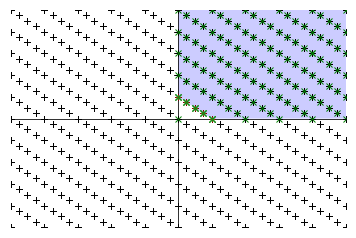
\includegraphics[width=0.8\linewidth]{conezoomout}
%\captionof{figure}{The Borel Graph of $b^2c$}
%\end{center}\vspace{1cm}


 \begin{center}
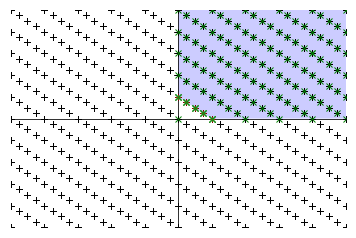
\includegraphics[width=0.7\linewidth]{conezoomout}
\captionof{figure}{\color{Green} The cone (blue), affine group (+) and affine semigroup (x) generated by $\mathcal{H}=\{ (4,0), (3,1), (2,2), (1,3), (0,4) \}$. Note the dashes on the axes are four units apart.}
\end{center}

\item The generating set of the lattice points 
$\mathcal{H} = \{ (4,0), (3,1), (2,2), (1,3),$ $(0,4) \}$ can be interpreted as generating the toric ring $K[T] = K[x^4, x^3y, x^2y^2, xy^3, y^4]$, where each $\mathbf{a_i} \in \mathcal{H}$ is an exponent vector for a monomial $m_i = \mathbf{x}^\mathbf{a_i} \in T$. In fact, this intuition is confirmed by the following theorem: 

\begin{theorem*}{\label{Affineiffaffinetoric}}\citep{Ene}
	Let $\mathcal{H} \subset \mathbb{N}^n $ and $H$ the affine semigroup generated by $\mathcal{H}$. Then $H$ is normal if and only if the toric ring $K[H]$ is normal, where $K$ is an algebraically closed field. 
\end{theorem*}

Thus, a normal toric ring is equivalent to the normal affine subgroup. The normality of the affine subgroup can be characterized by the following lemma. 

\columnbreak

\begin{theorem*}\textbf{Gordan's Lemma}\,\citep{Ene}\label{Gordan's Lemma}
\begin{enumerate}
	\item If $H$ is a normal affine semigroup generated by $\mathcal{H} \subset \mathbb{Z}^n$, then $H=\mathbb{Z}\mathcal{H} \cap \mathbb{R}_+ \mathcal{H}$.
	\item If $C$ is a finitely generated rational cone in $\mathbb{R}^n$, then $H=\mathbb{Z}^n \cap C$ is a normal affine subgroup.
\end{enumerate}
\end{theorem*}
\end{itemize} 


\psshadowbox[linewidth=1mm,framearc=0.1,linecolor=red,framesep=1em]{
\begin{minipage}[h]{0.9\linewidth}
\begin{theorem}{\label{Our theorem 1}}
	Let $K[B(u)] \subset K[x_1, \ldots, x_n]$ be a toric ring generated by the Borel set of a monomial $u \in K[x_1, \ldots, x_n] $. Then for all $\, m_i=\mathbf{x}^\mathbf{a_i} \in B(u)$, $K[B(u)\setminus m_i]$ is normal if and only if $a_i$ is a corner in the $n$-dimensional polygon formed by the exponent vectors of monomials in $B(u)$ in $\mathbb{R}^n$.
\end{theorem}
\end{minipage}}
\begin{proof}%I already had this open in another tab and was doing stuff to notation so I thought why not just do it now and save you the effort, but I just noticed you logged on now lol oh you already did it...cool...yeah I thought it would be too cumbersome to explain on groupme
% nah I understood what you meant, I wrote (n-1) but never clarified that $n$ was the degree of $u$, my fault mate - uploading it to Dropbox now... cool cool l8r
Let $\mathcal{H}$ be the set of exponent vectors on the monomials of $B(u)$, where $u$ is an $p$-degree monomial. Let $m_k$ with exponent vector $\mathbf{a}_k$ be pinched from $\mathcal{H}$. Let $\mathcal{H}' = \mathcal{H} \backslash \{\mathbf{a}_k\}$ and $H'$ the corresponding affine semigroup. 
	
Suppose $\mathbf{a}_k$ is a non-corner. Then since $B(u)$ is homogenous, the vectors in $\mathcal{H}$' lie in the same $(n-1)$-dimensional space, so $\mathbf{a}_k \in \mathbb{Z}\mathcal{H}' \cap \mathbb{R}_+ \mathcal{H}'$ and $\mathbf{a}_k \notin \mathcal{H}'$. By the contrapositive of the first part of Gordon's Lemma, $H'$ is non-normal.  %we can linearly combine them with coefficients in $\mathbb{Z}$ to form $\mathbf{a}_k$. Furthermore, the coplanarity also allows us to linearly combine them with coefficients in $\mathbb{R}_+$ to yield $\mathbf{a}_k$. Thus,

Suppose $\mathbf{a}_k$ was a corner point. If we take away $\mathbf{a}_k$ from $\mathcal{H}$,  $\mathcal{H}'$ will have a new set of corner points. It then follows that $\mathbb{R}_+\mathcal{H}' \cap \mathbb{Z}^n=H'$, and from the second part of Gordan's Lemma, it clear that $H'$ is normal. 


\end{proof} 

\begin{center}
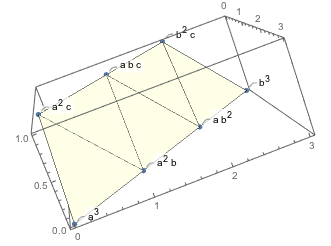
\includegraphics[width=0.6\linewidth]{b2clattice}
\captionof{figure}{\color{Green}The lattice points of $B(b^2c)$}
\end{center}

The corners in $B(b^2c)$ are $a^3, b^3, a^2c,$ and $b^2c$. These when pinched result in a new polygon. The non-corners such as $abc$ ``puncture" the polygon, resulting in its non-normality. 

\section*{\color{DarkSlateBlue}An extension to Rees Algebras}

\begin{definition}\textbf{Rees Algebra}{\label{Rees Algebra}}\\
	The \textit{Rees Algebra} of a Borel Ideal $\langle B(u) \rangle$ is the polynomial subring, and more precisely, the R-subalgebra, 
	\[ \mathcal{R} = K[x_1, \ldots, x_n][B(u)t] \subset K[x_1, \ldots, x_n][t] \] 
\end{definition}

Analogous to the toric ideal and toric map, we can define a \textit{Rees ideal} and a \textit{Rees Map}. The following theorem concerns the normality of the Rees algebra: 

%\begin{definition}\textbf{Rees Ideal}
%	Suppose $B(u) = \{ w_1, \ldots, w_s \}$ is a principal Borel set generated by $u \in K[x_1, \ldots, x_n]$. Let $\varphi$ be a surjective %ring homomorphism called the \textit{Rees Map}
%	\[ \varphi: K[x_1, \ldots, x_n][Y_{w_i}: w_i \in B(u)] \mapsto K[x_1, \ldots, x_n][B(u)t] \]
%	where 
%	\[ \varphi(Y_{w_i}) = w_i t \]
%Then $\mathcal{R}(\langle B(u) \rangle) =\,$Ker$(\varphi)$ is called the \textit{Rees Ideal} of  $B(u)$ 
%\end{definition}
%Note that the Rees map is just a toric map between rings in $n+1$ indeterminates. Thus, the Rees ideal is simply a toric ideal. With this observation, we can state our next result: 
\psshadowbox[linewidth=1mm,framearc=0.1,linecolor=red,framesep=1em]{%
\begin{minipage}[h]{0.9\linewidth}
\begin{theorem}\label{Main result 2}
	Let $m_i \in B(u)$ be a monomial. Then the toric ring $K[B(u) \setminus m_i]$ is normal if and only if the Rees algebra of $B(u) \setminus m_i$ is normal. Thus, those pinchings of a principal Borel ideal which lead to normal toric rings also lead to normal Rees algebras and vice versa. 
\end{theorem}
\end{minipage}}

This proof of this statement follows from the correspondence between corners and non-corners of the affine semigroup formed of the monomials that are pinched of the Rees Algebra, i.e. those with $t=1$, and affine semigroup associated with the toric ring, i.e. with $t=0$.

\begin{center}
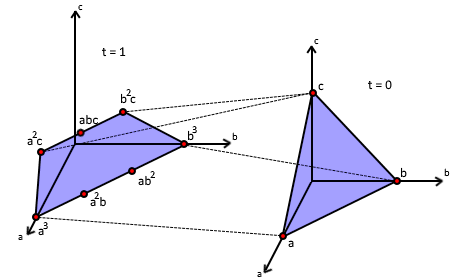
\includegraphics[width=0.70\linewidth]{reduction.png}
\captionof{figure}{\color{Green} Correspondence mapping for $B(b^2c)$.}
\end{center}

%\begin{proof}
%	Note that the Rees map is just a toric map between rings in $n+1$ indeterminates. We intend to know which pinchings create ``punctures" in the affine semigroup of the Rees Algebra, which is just a toric ring in $n+1$ variables. But since we only pinch those exponent vectors with $t=1$, the problem reduces to determining which points are corners and non-corners in the $t=1$ plane. But the $t=1$ plane is all the points which correspond to the generators of the affine semigroup associated with the toric ring. Thus, the corners and non-corners are identical between toric rings and Rees algebras. As a result, normality of the Rees algebra of a pinched principal borel is equivalent to the normality of its toric ring. 
	
% the affine semigroup is generated by the exponent vectors, and
%\end{proof}

\section*{\color{DarkSlateBlue}Further Directions}

Our further work involves developing results for toric rings of two Borel ideals, and studying the Koszulness of toric rings and Rees algebras of pinched principal Borel ideals. 

\begin{conjecture*}
	The rev-lex earliest non-normal, homogenous of degree $s$, two-Borel ideal $B(u,v)$, where $u, v \in K[x_1, \ldots, x_n]$ is $B(x^{s-2}_{1} x_{3}^{2}, x_{2}^s)$
\end{conjecture*} 

\begin{conjecture*}
	Let $B(u,v)$ be a homogenous non-normal two-Borel ideal. Then for all $ \, m: m\prec_{revlex}u$, define a chain of monomials $u=m_0 \rightarrow m_1 \rightarrow \ldots \rightarrow m_l = m$ where for all $ \, i: 1 \leq i \leq l, m_i = \frac{x_{k+1}}{x_k}m_{i-1}$ s.t $x_k \, | \, m$. If \, for all $ \, i: 1 \leq i \leq l, m_i$ and $v$ are coprime, then $B(m,v)$ is also non-normal.  
\end{conjecture*}

\begin{question*}
	Which pinched principal Borel ideals have toric rings that are Koszul? 
\end{question*}
This question remains open, and we have currently been trying to identify patterns in the data on Koszulness. 

\section*{\color{DarkSlateBlue}Acknowledgements}

We sincerely thank the SURF and Gregory S. Call Fellowships for supporting our research and Prof. Sosa for his patience, guidance, and for introducing the research problem. We also extend our heartfelt gratitude to the computer algebra system Macaulay2 and to Andy Anderson for allowing us access and help with the Amherst Computing Cluster. 

\color{DarkSlateBlue}
\bibliographystyle{plain}
\bibliography{Bibforposter}




%------------------------------------------------



%----------------------------------------------------------------------------------------

\end{multicols}
\end{document}